%
% Portuguese-BR vertion
% 
\documentclass{article}

\usepackage{ipprocess}
% Use longtable if you want big tables to split over multiple pages.
% \usepackage{longtable}
\usepackage[utf8]{inputenc} 
\usepackage[brazil]{babel} % Uncomment for portuguese

\sloppy

\graphicspath{{./pictures/}} % Pictures dir
\makeindex
\begin{document}

\DocumentTitle{Plano de Testes}
\Project{Core-MUSA}
\Organization{Universidade Estadual de Feira de Santana}
\Version{Build 2.0a}

\capa
\newpage

%%%%%%%%%%%%%%%%%%%%%%%%%%%%%%%%%%%%%%%%%%%%%%%%%%
%% Revision History
%%%%%%%%%%%%%%%%%%%%%%%%%%%%%%%%%%%%%%%%%%%%%%%%%%
\section*{\center Histórico de Revisões}
  \vspace*{1cm}
  \begin{table}[ht]
    \centering
    \begin{tabular}[pos]{|m{2cm} | m{7.2cm} | m{3.8cm}|} 
      \hline
      \cellcolor[gray]{0.9}
      \textbf{Date} & \cellcolor[gray]{0.9}\textbf{Descrição} & \cellcolor[gray]{0.9}\textbf{Autor(s)}\\ \hline
      \hline
      \small 10/11/2014 & \small Concepção do Documento & \small fmbboaventura \\ \hline      
     \small 16/11/2014 &
      \begin{small}
        \begin{itemize}
          \item Plano de Teste da Memória de Instrução;
        \end{itemize}
      \end{small} & \small mtcastro \\ \hline
    \end{tabular}
  \end{table}

\newpage

% TOC instantiation
\tableofcontents
\newpage

%%%%%%%%%%%%%%%%%%%%%%%%%%%%%%%%%%%%%%%%%%%%%%%%%%
%% Document main content
%%%%%%%%%%%%%%%%%%%%%%%%%%%%%%%%%%%%%%%%%%%%%%%%%%
\section{Introdução}

  \subsection{Objetivo}
  Este documento tem como objetivo descrever os casos de teste dos componentes do processador de propósito geral MUSA.
  
  \subsection{Visão Geral do Documento}
  \begin{itemize}
    \item Sessão 2: REVER.
    \item Sessão 3: relata a lista dos casos de teste do projeto.
    % \item Referências: provê uma lista completa de todos os artefatos referenciados nesse documento.
  \end{itemize}
  
  \subsection{Representação Simbólica [PARTE DO DOCUMENTO DE USE CASES!!]}
  A Figura \ref{fig:uc_exemple} ilustra a simbologia utilizada para representar operações que devem ser realizadas pelo sistema. A Figura \ref{fig:actors} ilustra as duas simbologias utilizadas para representar os Atores do sistema. Um ator, dentro do escopo desta descrição, pode ser identificado como um módulo \textit{top level}, ou como um elemento de entrada e saída (botões, sensores, displays, etc).
  
  \FloatBarrier
  \begin{figure}[H]
    \centering
    
\includegraphics[width=0.25\textwidth]{uc_exemple.png}
    \caption{Exemplo de Caso de Uso.}
    \label{fig:uc_exemple}
  \end{figure}  
  
  A simbologia usual para representação de um Ator é apresentada na Figura \ref{fig:actor_exemple}, no entanto, para representar módulos incorporados que outrora deveriam utilizar a mesma simbologia, utiliza-se a representação ilustrada nas Figuras \ref{fig:ipcore_exemple} e \ref{fig:ipcore_single_exemple}, definida por convenção. Este elemento, em geral, está associado aos módulos do sistema, ou IP-cores que de terceiros incorporados ao mesmo. Esta simbologia ainda foi divida, tendo em vista representar instâncias únicas (Figura \ref{fig:ipcore_single_exemple}), ou múltiplas (Figura \ref{fig:ipcore_exemple}) de um determinado componente. 
  
  \FloatBarrier
  \begin{figure}[H]
    \centering
    \begin{subfigure}[b]{0.3\textwidth}
      \centering
      
\includegraphics[width=0.25\textwidth]{actor_exemple.png}
      \caption{Ator do Sistema.}
      \label{fig:actor_exemple}
    \end{subfigure} 
    \begin{subfigure}[b]{0.3\textwidth}
      \centering
      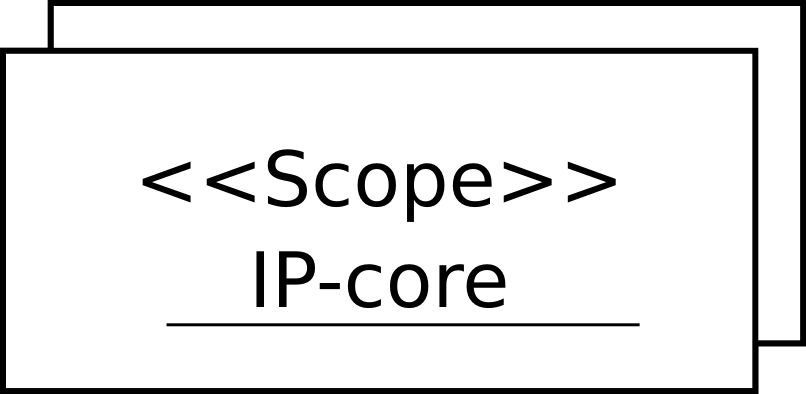
\includegraphics[width=0.6\textwidth]{ipcore_exemple.png}
      \caption{Instância múltipla de um IP.}
      \label{fig:ipcore_exemple}
    \end{subfigure}
    \begin{subfigure}[b]{0.3\textwidth}
      \centering
      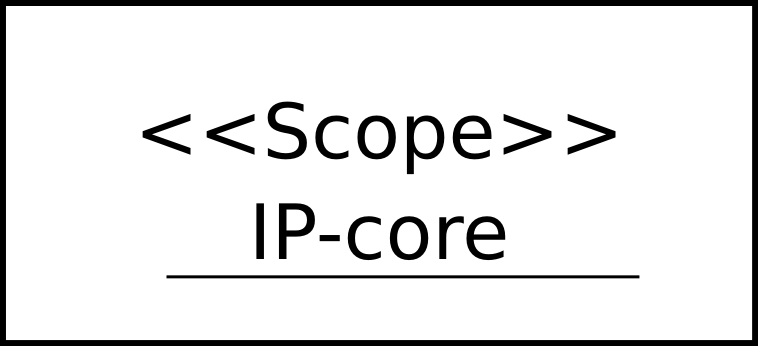
\includegraphics[width=0.6\textwidth]{ipcore_single_exemple.png}
      \caption{Instância de um IP.}
      \label{fig:ipcore_single_exemple}
    \end{subfigure}
    \caption{Simbologia utilizada na implementação dos Casos de Uso.}
    \label{fig:actors}
  \end{figure}
  
  O projetista responsável por interpretar os diagramas não deve confundir-se no momento de interpretar as simbologias de atores. A representação alternativa, não implica que o módulo será instanciado no subsistema em questão, mas sim que os recursos providos por este \textit{core} são necessários para garantir o seu funcionamento.
  
  \subsection{Definições, Acrônimos e Abreviações}
  \FloatBarrier
    \begin{table}[H] 
      \begin{center}
        \begin{tabular}[pos]{|m{2cm} | m{8cm}|} 
          \hline 
          \cellcolor[gray]{0.9}\textbf{Termo} & \cellcolor[gray]{0.9}\textbf{Descrição} \\ \hline
          TC & Caso de Teste  \\ \hline
          SB & Sub-fluxo \\ \hline
          FS & Fluxo Secundário \\ \hline
          NFR & Requisito Não Funcional \\ \hline
          FR & Requisito Funcional \\
          \hline
        \end{tabular}
      \end{center}
    \label{tab:definicoes}
    \end{table}

  \section{Atores do Sistema [PARTE DO DOCUMENTO DE CASO DE USO!!]}
  
  \section{Casos de Teste}
  Esta sessão apresenta o conjunto de TC realizados para a implementação dos testes do projeto Core-MUSA. As sessões a seguir foram divididas e nomeadas utilizando a nomenclatura abreviada [TC (NÚMERO DO TC)] seguido de uma breve descrição em forma de título.

  \testcase{ULA}
A ULA tem como objetivo principal realizar operações logicas e aritimeticas, onde algumas delas estão ligadas diretamente a flags informativas ou de erros.
  
  \inputs
  	\begin{itemize}
     \item Operando 1;
     \item Operando 2;
     \item Sinal de identificação da operação;
     \end{itemize}
    
  \actions
  \begin{itemize}
     \item Realizar a operação solicitada;
     \item Ativar os sinais de saida de dados e de flags, caso ocorram;
    \end{itemize}
  
  \results
  	\begin{itemize}
     \item Valor de 32 bits relativos ao resultado da operação;
     \item Sinal de flag, caso ocorram;
    \end{itemize}
  
  % descricao do fluxo principal de eventos
  \begin{mainflow}
    \item As funcionalidades serão testadas na seguinte ordem de acordo com o sinal de identificação: ADD, ADDI, SUB, SUBI,
AND, ANDI, OR, ORI, MUL, DIV, CMP, NOT;
    \item Os valores ultilizados para os operandos serão adquiridos de forma aleatória;
    \item Cada funcionalidade será testada 100 vezes;
    \item Serão testados os seguintes casos de flags auxiliares: Equals ,Above;
    \item Serão testados os seguintes casos de flag de erro de forma proposital: Overflow;
    \item As flags serão testadas com a ultilização de uma saida de controle temporária para os sinais;
  \end{mainflow}
  
  % descricao do fluxo secundário (quando existir)
  \begin{secondaryflow} 
    \sfitem{Título do Fluxo Secundário}
    \begin{enumerate}
      \item Liste aqui as etapas do fluxo secundário;
    \end{enumerate}
    \sfitem{Título do Fluxo Secundário}
    \begin{enumerate}
      \item Liste aqui as etapas do fluxo secundário;
    \end{enumerate}
  \end{secondaryflow}  
  
  
  
  \testcase{Memória de Instrução}
O objetivo deste teste é garantir que os registradores responsáveis por armazenar as instruções do programa  estejam lendo as informações corretas na posição correta.
  
  \inputs
  	\begin{itemize}
     \item Endereço de Instrução;
     \end{itemize}
    
  \actions
  \begin{itemize}
     \item Busca um instrução na posição informada no endereço;
    \end{itemize}
  
  \results
  	\begin{itemize}
     \item Confirmação da veracidade dos dados informado na saída;
    \end{itemize}
  
  % descricao do fluxo principal de eventos
  \begin{mainflow}
    \item A memória de instrução recebe um endereço, a instrução
Relacionada é buscada e passada adiante;
    \item A entrada será um código de endereço aleatório  de 18 bits;
    
    \item Será testada 20 vezes;
    \item A condição de testes é que o valor contido nos registradores de instrução seja igual ao valor associado ao endereço de instrução do programa de teste;
    
    \item Critério de aceitação é acertos igual ou maior 99\% do total de casos de teste;
    \item As flags serão testadas com a ultilização de uma saida de controle temporária para os sinais;
  \end{mainflow}

% Optional bibliography section
% To use bibliograpy, first provide the ipprocess.bib file on the root folder.
% \bibliographystyle{ieeetr}
% \bibliography{ipprocess}

\end{document}
